%!TEX root = ../dissertation.tex
\chapter{Aperture effects in Stellar Mass Estimates}

\label{ch:acm}
\newpage

\section{Introduction}

In this chapter we investigate methods of constraining the star formation histories and stellar masses of galaxies where galaxy spectra are available. In particular, we look at the largest galaxy catalog of estimated stellar masses, star formation rates and gas metallicities (the MPA-JHU catalog; {\bf NEED CITATION}) obtained for the Sloan Digital Sky Survey (SDSS) Legacy Survey. The MPA-JHU catalog has, over the last decade and a half, been one of the most influential and widely-used catalogs in the fields of galaxy formation and evolution. Here we test a fundamental assumption of the catalog, which is that spectroscopic measurements of the central region of the galaxy yield sufficient information to constrain star formation histories and stellar masses for the galaxy as a whole.\textbf{MRB says: You need to describe briefly why we want to measure
these quantities. Call back to Chapter 0. }\\


The SDSS spectra are obtained for multiple objects at a given time. This is done by connecting the spectrographs to fiber optic cables which are plugged into an aluminum plate that is placed in the telescope's focal plane. These optical fibers have a fiber diameter of $3''$. Thus for each galaxy in the SDSS, while photometry is available for the entire galaxy, spectra are available only for the region of the galaxy contained within this $3''$ angular aperture. Thus, the fraction of the galaxy falling within the aperture may vary widely with the redshift of this galaxy. I describe below how the MPA-JHU catalog approached this problem.\\
The stellar masses and star formation histories in the catalog are obtained by looking at two key spectral indicators of starbursts and age of a galaxy: the Balmer $H\delta_{\rm A}$ absorption line index and the $D_{n}4000$ break index, both of which are relatively insensitive to the metallicity-age degeneracy issue that spectral indicators in the redder side of the spectrum are limited by. {\bf Because they are both measurements over a narrow range of wavelengths, that are similar to each other, and are independent of the absolute flux, they are designed to be insensitive to dust extinction within the galaxy}. Using the distribution of the observed galaxies in the $H\delta_{\rm A}-D_{n}4000$ plane and by employing Stellar Population Synthesis (SPS) models by \citet{bruzual_stellar_2003-1} to model the evolution of galaxies in this plane, they are able to infer a mass-to-light ratio in the $z$-band \citep{kauffmann_stellar_2003} for every point in this phase space. From here, it is a short step to using the luminosity of the entire galaxy to infer the stellar mass and star formation history of the galaxy.\\
However, this methodology can be problematic when the mass-to-light ($M/L$) ratio of the central part of a galaxy is not representative of the entire galaxy. This can be an issue where there are distinct bulge and disk components, such as for luminous spiral galaxies. However, with the availability of spatially resolved spectra for galaxies from IFU (Integral Field Unit) based surveys such as MaNGA(Mapping Nearby Galaxies at Apache Point \citep{bundy_overview_2014}), SAMI (Sydney-Australian-Astronomical-Observatory Multi-object Integral-Field Spectrograph \citep{bryant_sami_2015}), MUSE (Multi Unit Spectroscopic Explorer \citep{bacon_muse_2015}) and CALIFA (Calar Alto Legacy Integral Field Area Survey) \citep{sanchez_califa_2012}, we can actually put this question to the test and quantify the effect of aperture size on the SDSS stellar masses. We use MaNGA, the largest IFU-based survey thus far, which is based on SDSS, and ask the following questions: At any given redshift in the local Unverse, how does the position of the galaxy in the $H\delta_{A}-D_{n}4000$ plane as measured using a $3''$ aperture compare to using a full aperture, i.e. spectra from all the spatially resolved regions in the galaxy.\\ 

\subsection{The SDSS spectra}
Describing the SDSS spectrograph and $3''$ fiber diameter. References: \citep{smee_multi-object_2013} (\bf York et al citation).\\
The galaxy spectra in SDSS are obtained through $3''$ diameter fibers. The rest-frame wavelength range of the spectra at the median redshift is from 3500 \AA to 8500 \AA with a spectral resolution $$R = \frac{\Delta \lambda}{\lambda} \approx 2000$$. The spectra are calibrated using observations of F stars in each $3$ degree field.

\subsection{The MPA JHU Catalog}
Introduction to and describing the importance of the largest catalogue of galaxy stellar masses \citep{kauffmann_stellar_2003}, star formation rates \citep{brinchmann_physical_2004} and gas metallicities \citep{tremonti_origin_2004} thus far. Including major results that rely on said SFR's.\\
{\bf MRB says: Then you need to mention some major results that depend
on the MPA-JHU catalog measurements of this quantity, just a couple of 
highlights from the later section. }{\bf TBD:  Kewley et al 2006 (host galaxies of AGN's); Clowe 2006 A Direct Empirical Proof of the Existence of Dark Matter; Elbaz et al 2007 The reversal of the star formation-density relation in the distant
universe; Kewley 2008 Metallicity Calibrations and the Mass-Metallicity Relation for Star-forming Galaxies; Peng et al 2010(mass and environments as drivers etc); Kauffmann 2013 A re-examination of galactic conformity and a comparison with semi-analytic models of galaxy formation}.\\
.....................

The MPA-JHU catalog was developed as a result of a joint collaboration between MPA and JHU right after the SDSS Data Release 1(DR1) of spectroscopic observations. Using the previously mentioned spectral indicators ($D_{\rm n}4000$ and $H{\delta_{\rm A}$) and broadband photometry from SDSS, they developed a method to derive maximum likelihood estimates of the stellar mass of a galay, the attenuation of optical light by dust and the fraction of stars in a galaxy formed in recent bursts.  The dataset they used was 120,808 galaxies drawn from the SDSS DR1. 



\begin{figure}
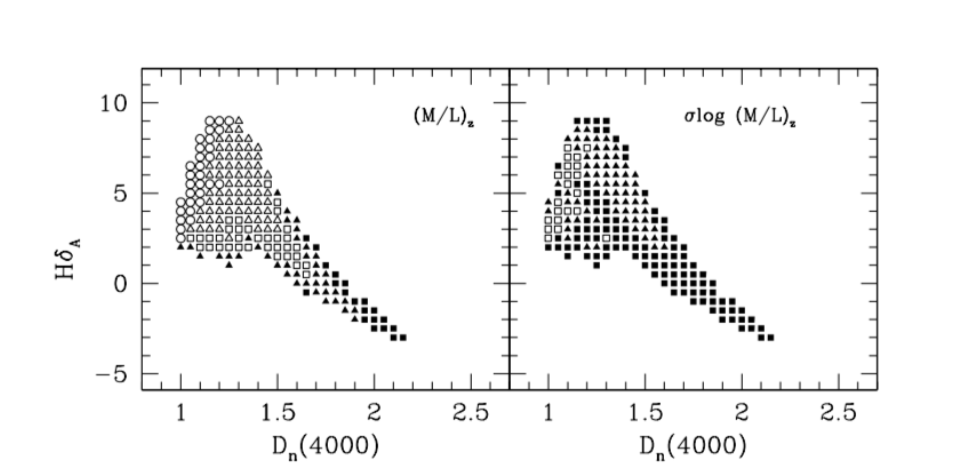
\includegraphics[width=\textwidth]{figures/Kauffmann_grid}
\caption[Short figure name.]{The \citet{kauffmann_stellar_2003} grid to infer M/L ratios from the $h\delta_{A}-D_{n}4000$ plane
\label{fig:kauff_grid}}
\end{figure}

\section{The $H\delta_{\rm A}-D_{n}4000$ plane}

Two powerful spectral diagnostic tools that are valuable in constraining stellar masses and star formation histories in galaxies are the Balmer $\delta$ absorption line index and the $D_{n}4000$ break index in the optical spectrum of a galaxy \citep{kauffmann_stellar_2003}. One of the key issues in spectral indicators for starbursts is the existence of the age-metallicity degeneracy in stellar populations \citep{worthey_comprehensive_1994}. The heavier element lines are often prominent in both early type as well as metal rich galaxies and the two are hard to distinguish in terms of interpretation as older stellar populations exhibit metal richness as well and without accurate modeling of the chemical evolution of galaxies, it is difficult to ascertain the reason. The Balmer $H\alpha$ and $H\beta$ are sensitive to the effects of metallicity as well. However both the Balmer $H\delta$ absorption line as well as the $D_{n}4000$ break occurring in the continuum are both in a bluer region of the spectrum relatively unaffected by metallicity constraints and together they form a powerful diagnostic tool to constrain the mass-to-light ratios of galaxies. 

\subsection{Measuring the $D_{\rm n}4000$ index}
\begin{figure}
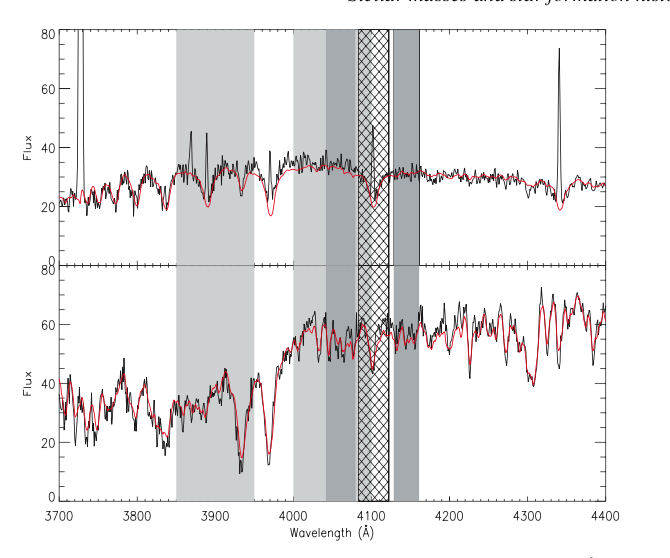
\includegraphics[width=\textwidth]{figures/spectra_placeholder.png}
\caption[Short figure name.]{ PLACEHOLDER FIG; TBD: A figure showing D4000 and Hdelta breaks in spectra for early/late-type galaxies as well as the bimodality in D4000
\label{fig:early_late_type}}
\end{figure}
The most obvious discontinuity in the spectrum of a galaxy is often the $D_{n}4000$ break \citep{1999ApJ...527...54B}, which is a consequence of the absorption into electronic excited states by neutral and partially ionized metals whose lines happen to overlap in the region just blueward of 4000 \AA.  Older stellar populations have spectra dominated by relatively cool giant stars, and under these conditions the partially ionized metal lines are strong. Younger stellar populations have spectra dominated by hot stars, for which these lines are weaker. In addition the break
depends on stellar metallicity, exhibiting some of the same age-metallicity degeneracy that afflicts most spectroscopic indicators.\\ 

This break was defined in by \citet{bruzual_a._spectral_1983-2} as the ratio of the average flux density $F_{\rm \nu}$ in two bands that span \textasciitilde200 \AA on either side of 4000 \AA. \citet{1999ApJ...527...54B} defined a narrow band definition for the same where the bands that are now 100 \AA wide with 3850 \AA - 3950 \AA as the ``blue continuum" and 4000 \AA - 4100 \AA as the ``red continuum". The bandpass used in \citet{kauffmann_stellar_2003} (\ref{fig:early_late_type}) is the same as the one introduced by \citet{1999ApJ...527...54B} and their motivation for doing so is that the narrow definition is more insensitive to reddening effects. I reproduce these measurements using the same narrow band definition.\\


\section{Manga Overview}
Citations: \citep{bundy_overview_2014}

\subsection{Introduction to Integral Field Spectroscopy}
What is Integral Field Spectroscopy? What is an Integral Field Unit? 

\subsection{The MaNGA IFU Design}
What is a spaxel? \citep{drory_manga_2015}

\section{Data}
\subsection{MaNGA Target Selection and DRP}
Primary and Secondary Samples. NSA redshifts/Luminosity cut.

\subsection{Our Sample}
The most recent MaNGA product launch, MPL-$8$, which was announced in November $2018$, containing products based on galaxy and stellar library observations from March $2014$ - July $2018$ serves as the source of our sample. It contains $950$ plates - $6779$ data cubes and $20649$ stellar library stars. Out of these, $6468$ are galaxies with measured NSA redshifts. These are representative of all the IFU sizes (list them: 19,37... 127) and span a redshift range upto $z = 0.15$.\\
For each galaxy observation, depending on the IFU bundle size (say $N_{X}$, $N_{Y}$ each describing a position $0.5$" from the previous spaxel), we have ($N_{X}$, $N_{Y}$) spectra which span $4563$ wavelength points. 

\section{Methods}

\subsection{Variable Aperture Measurements}
For any given datacube, we can determine which spaxels fall within an aperture radius of $R$ arc-seconds as follows. As each spaxel spans a width of $0.5$" in along the ``X" and ``Y" direction, at any point $(x,y)$ in the IFU image, the distance in arc-seconds of the centre of a spaxel from the central spaxel $(x_{c},y_{c})$ in the IFU would be:
$$ d = (r(x,y) - r(x_{c},y_{c})) = \sqrt{(0.5*x)^2 + (0.5*y)^2} $$
Thus, for every spaxel in the IFU, where $d<=R$, that part of the galaxy would fall within the aperture and hence, we would include that spaxel in the measurement of whichever spectral index. Using this, for instance, we can simulate the SDSS fiber measurement, i.e.,  what the $1.5$" aperture radius used in SDSS would see versus the total galaxy or what we call a ``full aperture" measurement.

\subsection{Variable Redshift Measurements}
One can alternately pose this question in terms of redshift. For all galaxies whose redshift $z_{\rm obs}$ is less than the redshift we are interested in, $z_{\rm cutoff}$, we can ask the question: if we shift the said galaxy to the said cutoff point, where would its location on the $H\delta_{\rm A}$ - $D_{\rm n}4000$ plane be? How offset is this from the ``full aperture" measurements?\\

Transverse angular distance varies with redshift as follows:
$$D_{\rm A}(z) = \frac{D_{\rm M}(z)}{1+z} $$,
where $D_{\rm M}(z)$ is the co-moving distance at redshift z.

So when a galaxy at $z_{\rm obs}$ is shifted to $z_{\rm cutoff}$ the new distance $d_{\rm new}$ of spaxel $(x,y)$ from the central spaxel $(x_{c},y_{c})$ relates to the old distance thus:
$$ d_{\rm new} = \frac{(1+z_{\rm cutoff})\times D_{\rm M}(z_{\rm obs}) \times d}{(1+z_{\rm obs}) \times  D_{\rm M}(z_{\rm cutoff})} $$

Using the above, we can now figure out the spaxels that would fall within a $3''$ diameter aperture (say) at not only the observed redshift but also any redshift where we would like to collectively observe the behavior of the offset with a full aperture measurement in the $H\delta_{\rm A}$ - $D_{\rm n}4000$ plane.


\begin{figure}
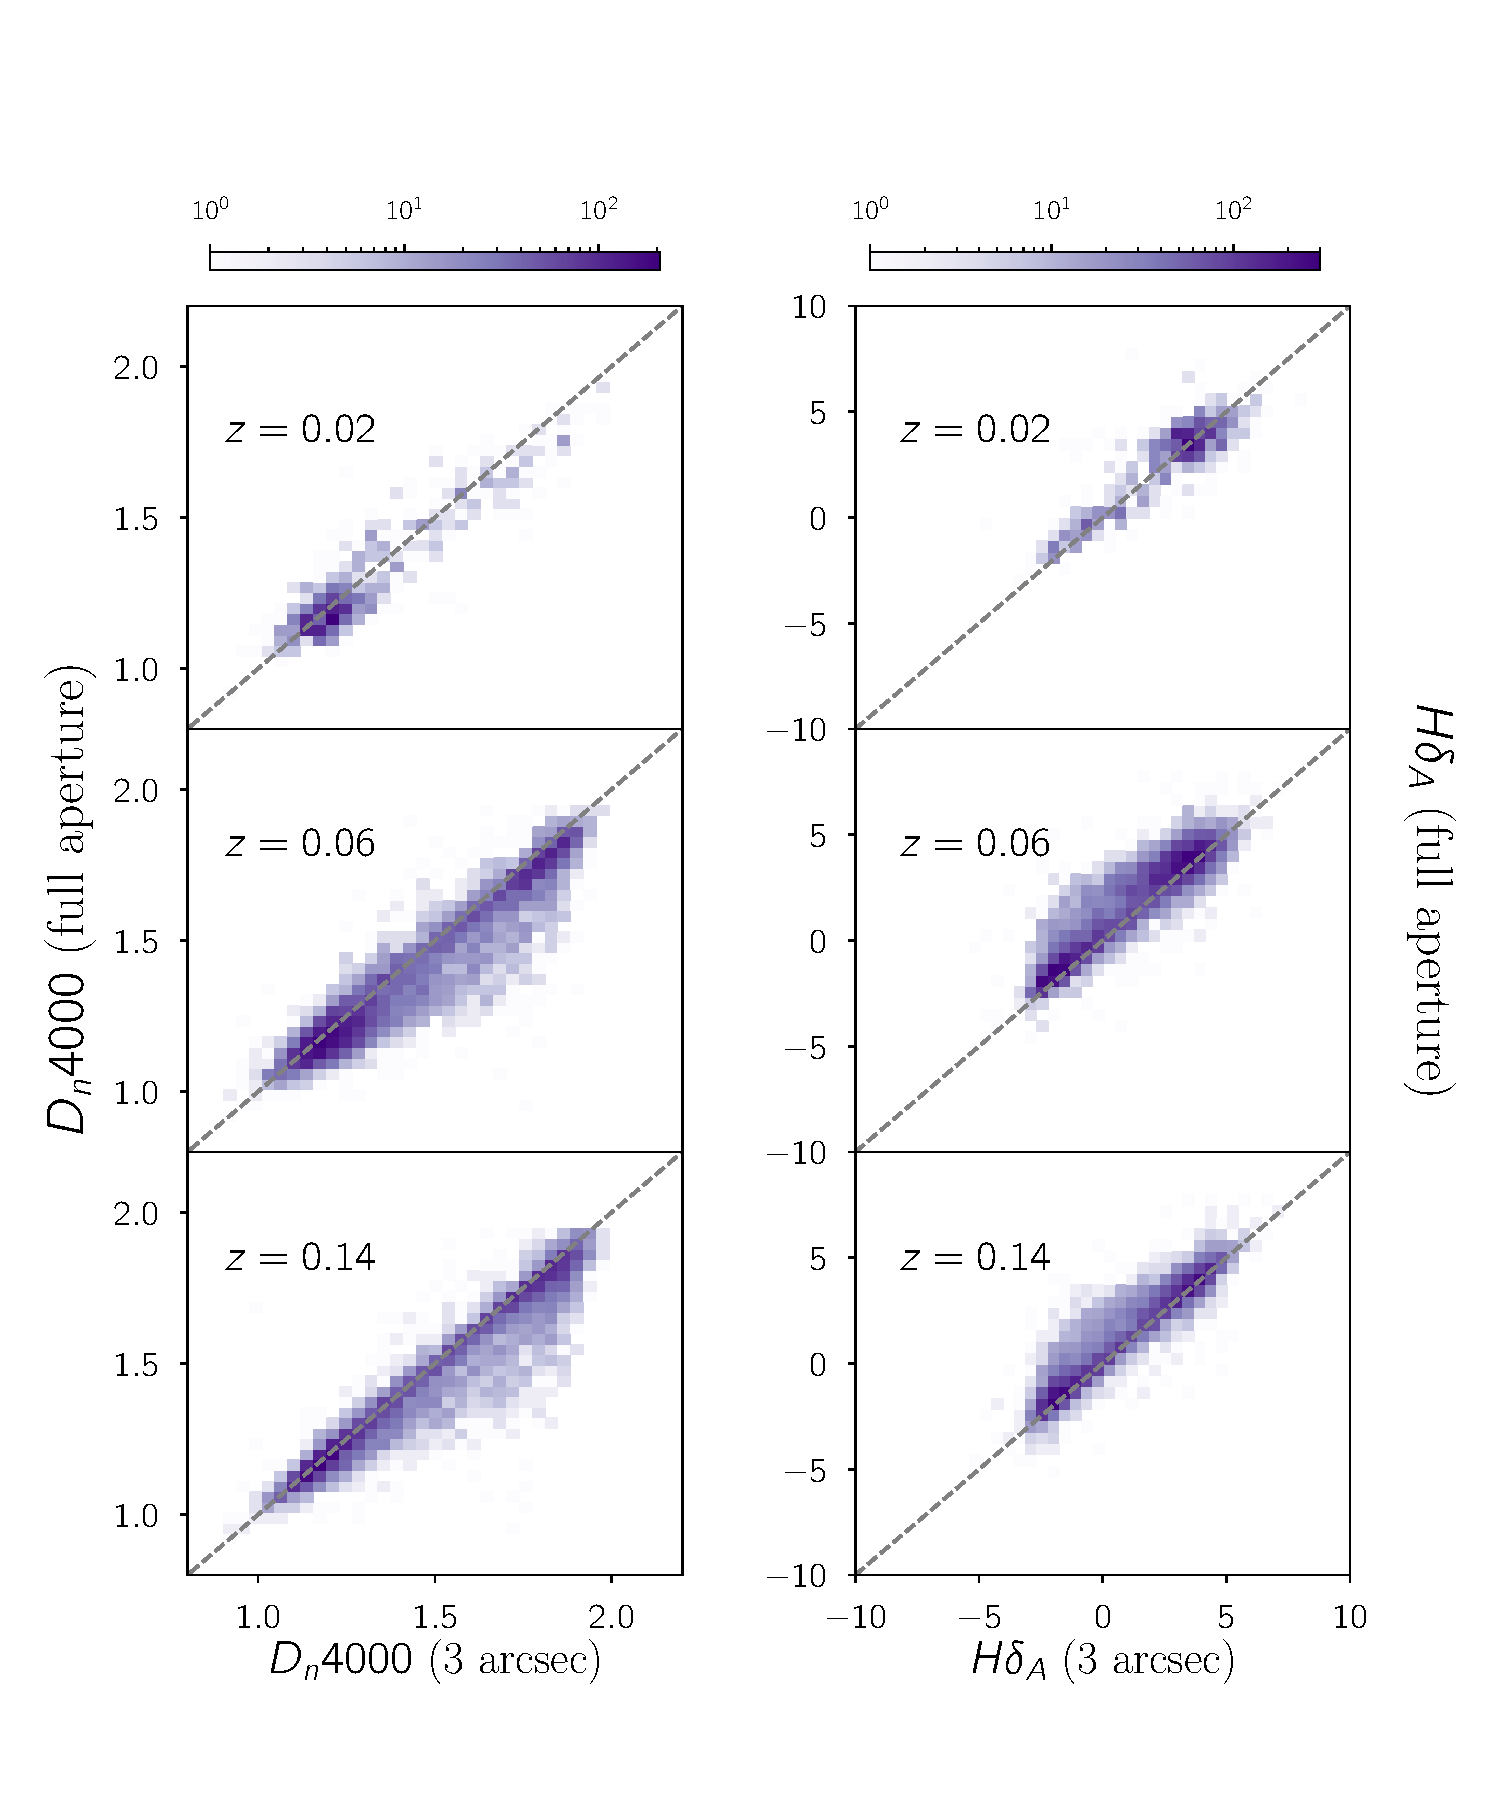
\includegraphics[width=\textwidth]{figures/full_aperture_comparisons.pdf}
\caption[Short figure name.]{ The $D_{n}4000$, $h\delta_{A}$ indices measured at $z = 0.02,0.06,0.14$ with a $3''$ aperture compared to the full aperture measurement
\label{fig:myInlineFigure}}
\end{figure}


\subsection{$H\delta_{\rm A}$, $D_{\rm n}4000$ Measurements within Apertures}
To get the $H\delta_{\rm A}$ and $D_{\rm n}4000$ index measurements for any aperture, we first redshift-correct the spectra obtained from all the spaxels within the aperture to rest-frame. As both the equivalent width of the Balmer $H\delta$ line as well as the $D_{n}4000$ break rely on the continuum as well as a ratio of fluxes in the case of the latter, we add up the spectra of the spaxels that fall within any aperture before estimating either. We then follow the procedure described in Section $2.2$ to calculate the indices. (In a footnote: the code for this is publicly available at --provide github link--.)


\begin{figure}
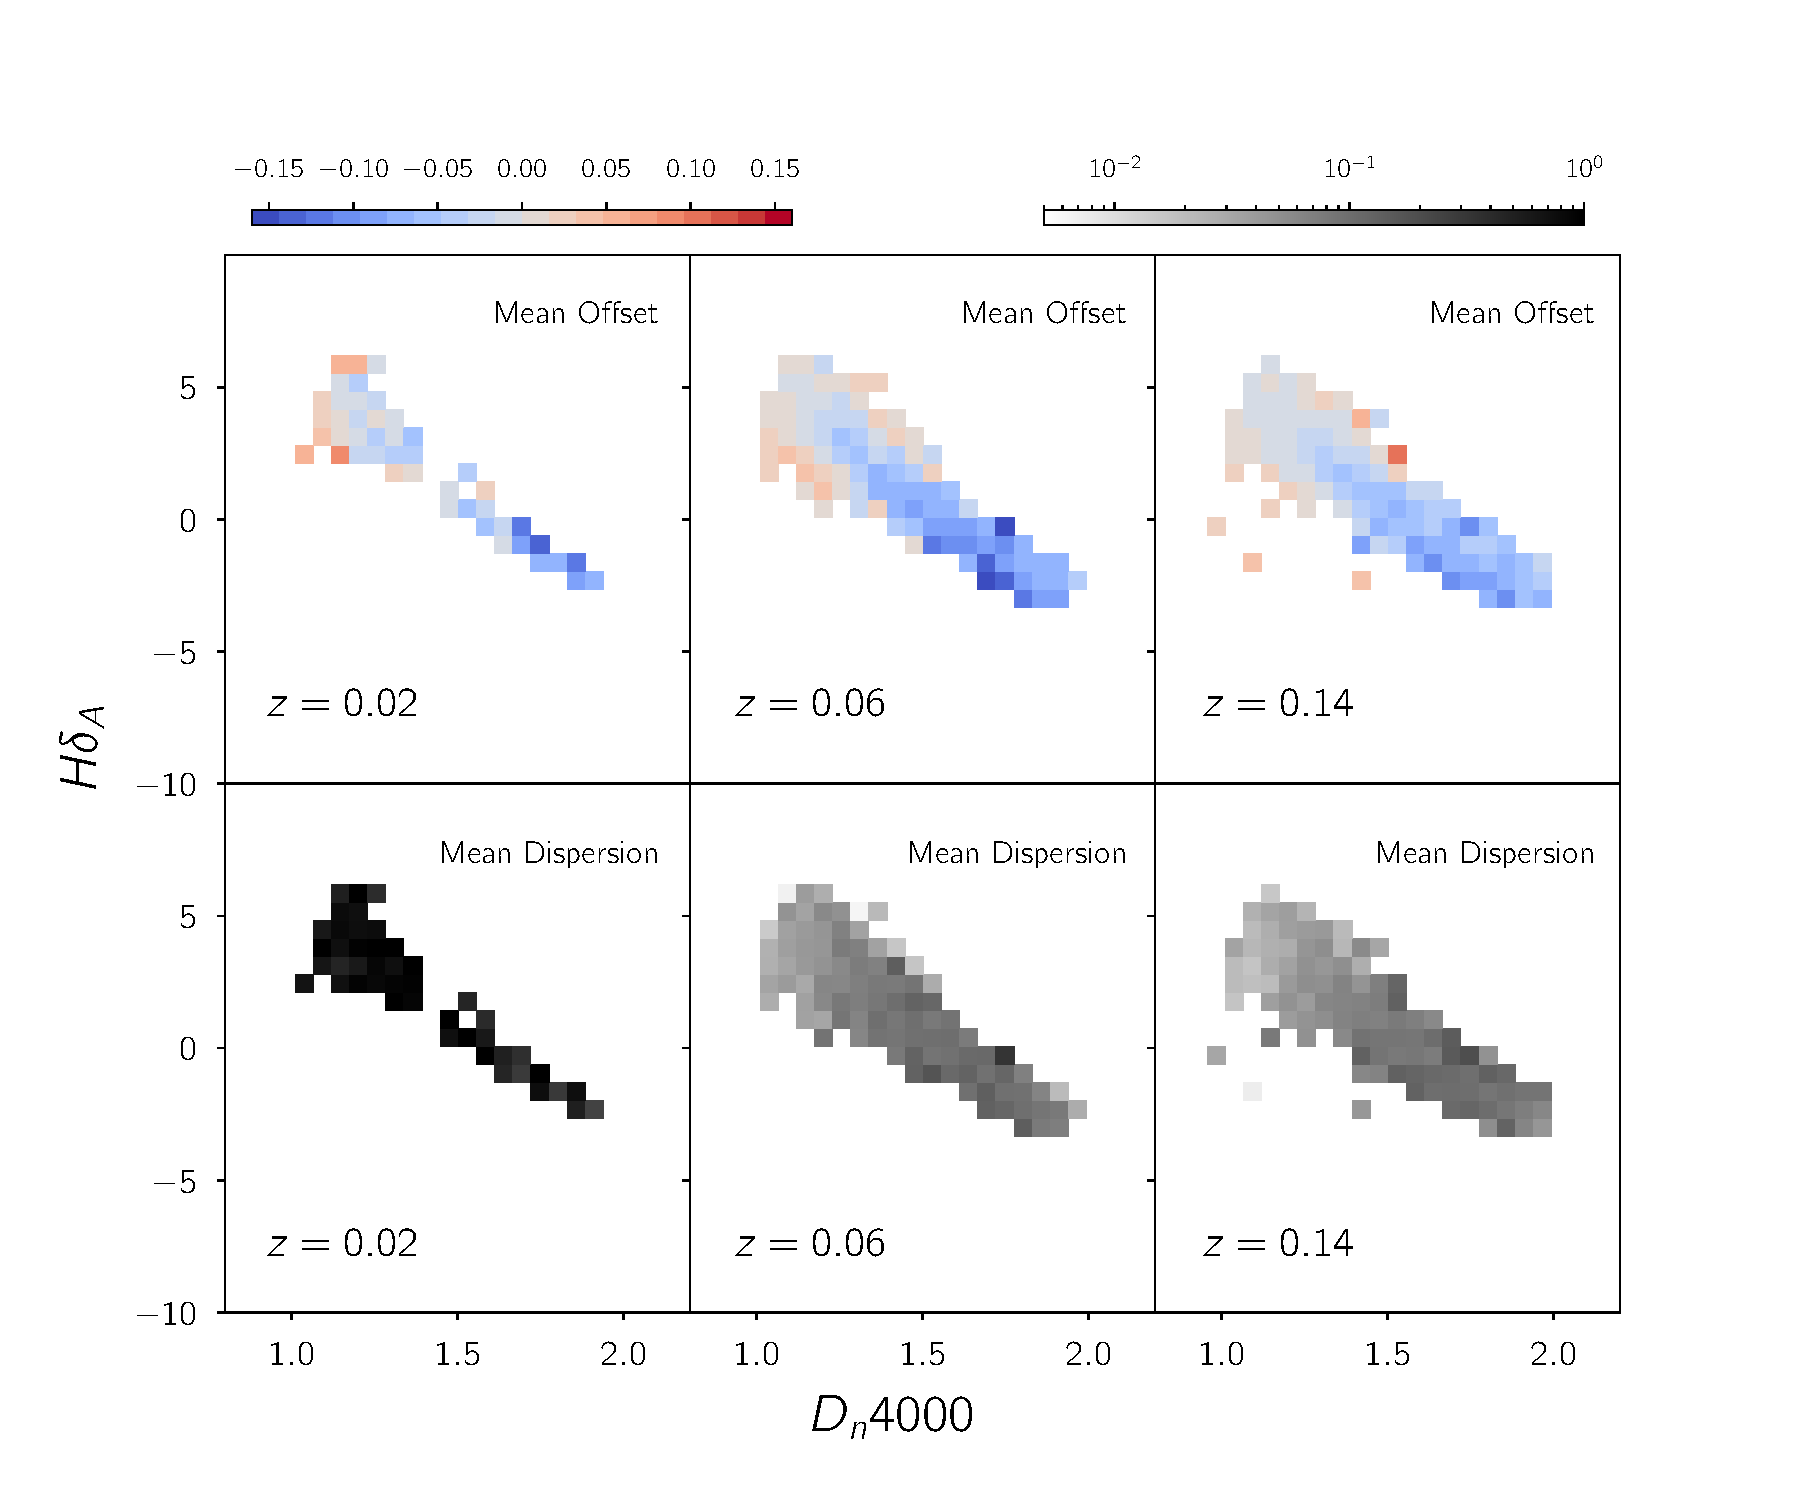
\includegraphics[width=\textwidth]{figures/dn4000_full_aperture_comparisons.pdf}
\caption[Short figure name.]{ The mean offset and dispersion in the $D_{n}4000$ index measured at $z = 0.02,0.06$ and $0.14$ with a $3''$ aperture from the full aperture measurement
\label{fig:myInlineFigure}}
\end{figure}



\section{Results}


\begin{figure}
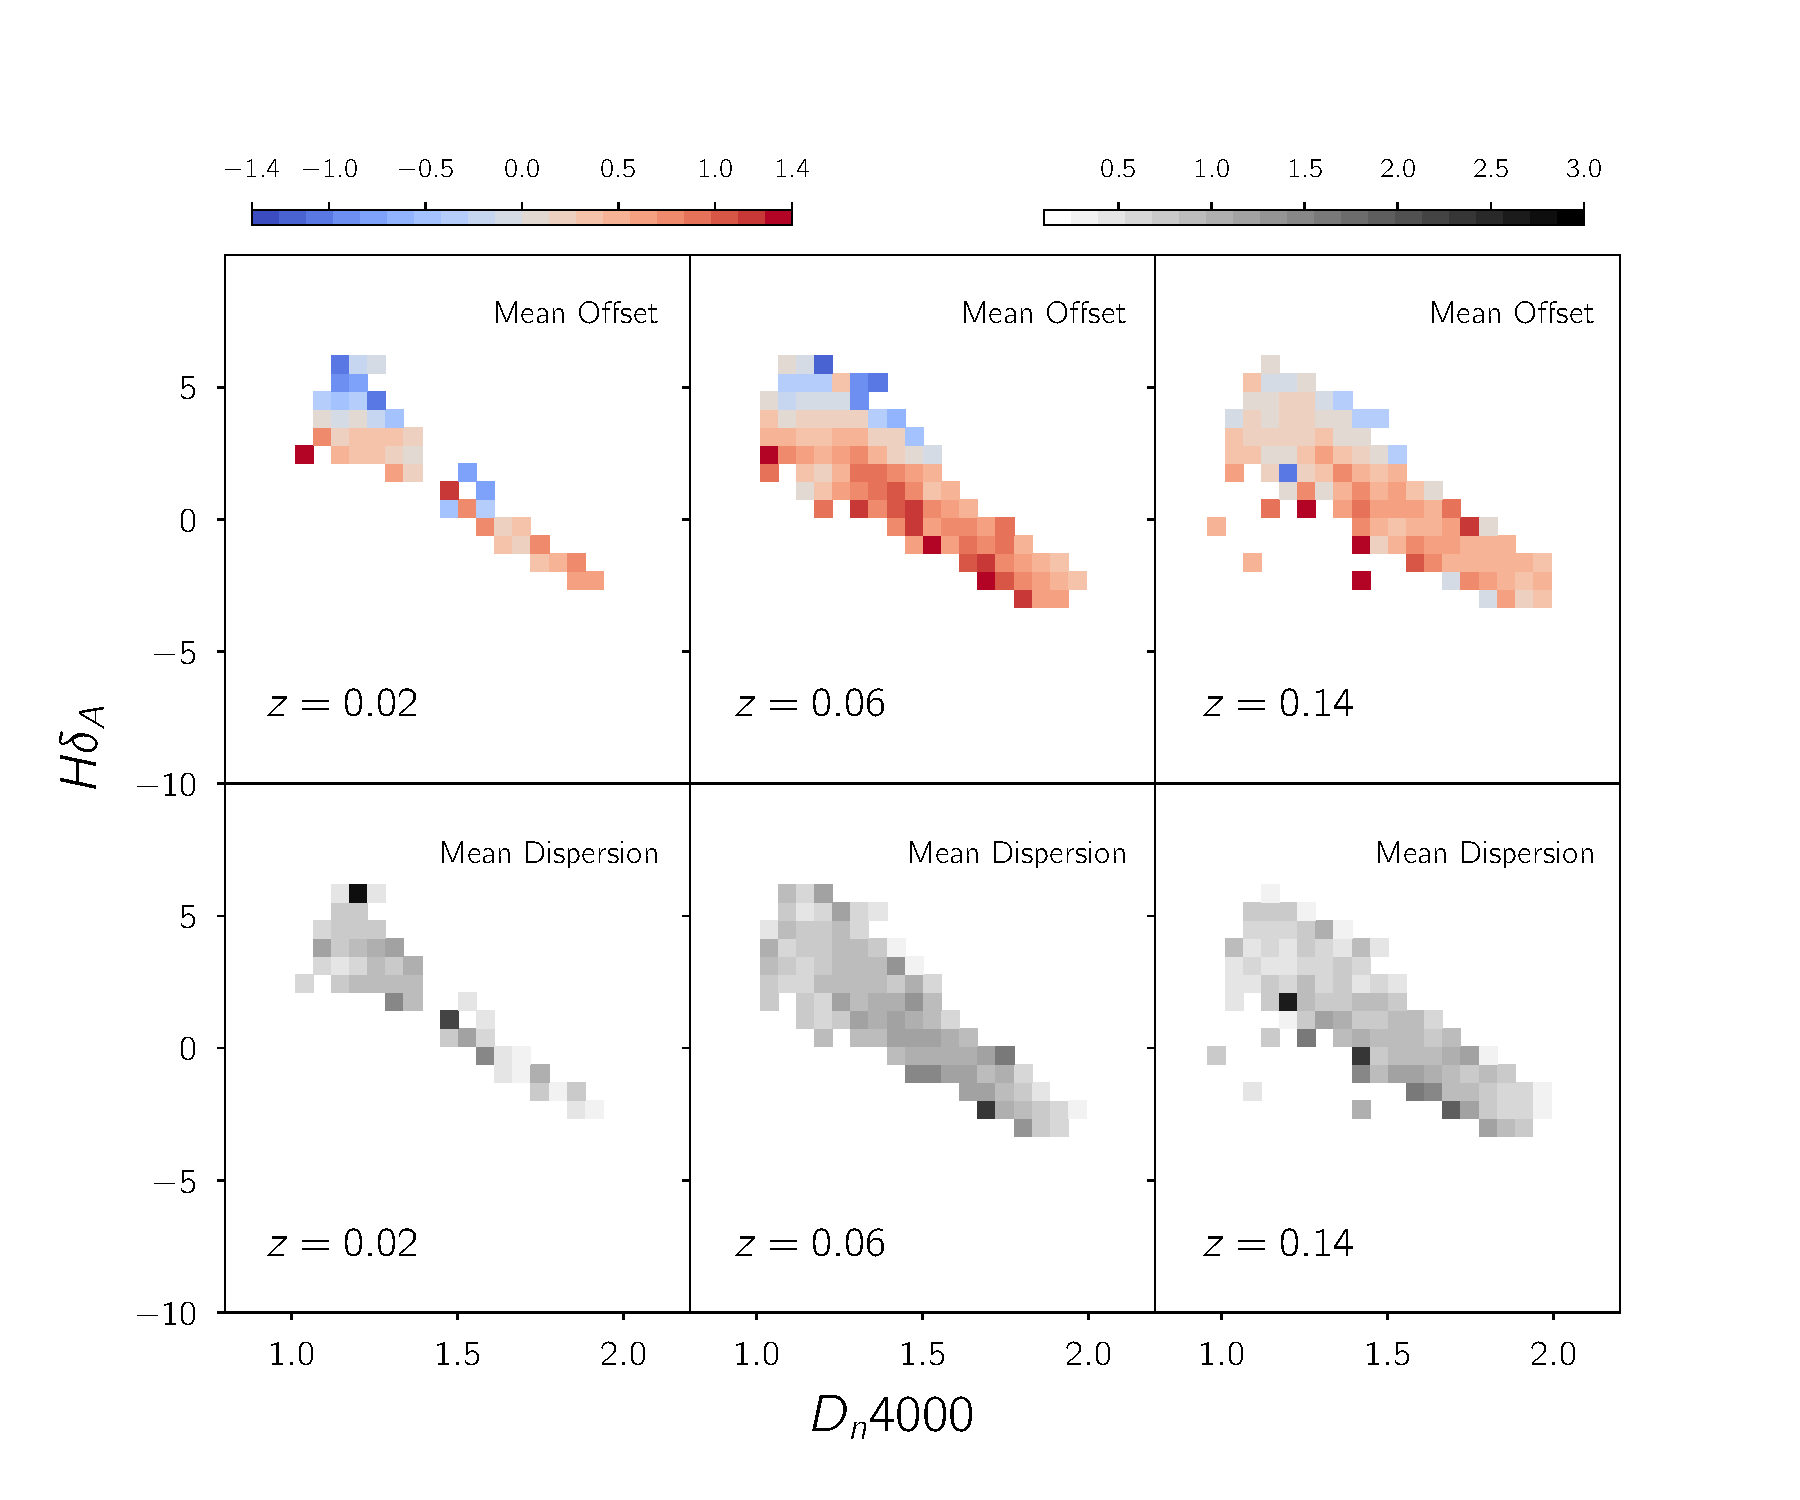
\includegraphics[width=\textwidth]{figures/hdelta_full_aperture_comparisons.pdf}
\caption[Short figure name.]{ The mean offset and dispersion in the $h\delta_{A}$ index measured at $z = 0.02,0.06$ and $0.14$ with a $3''$ aperture from the full aperture measurement 
\label{fig:myInlineFigure}}
\end{figure}

\begin{figure}
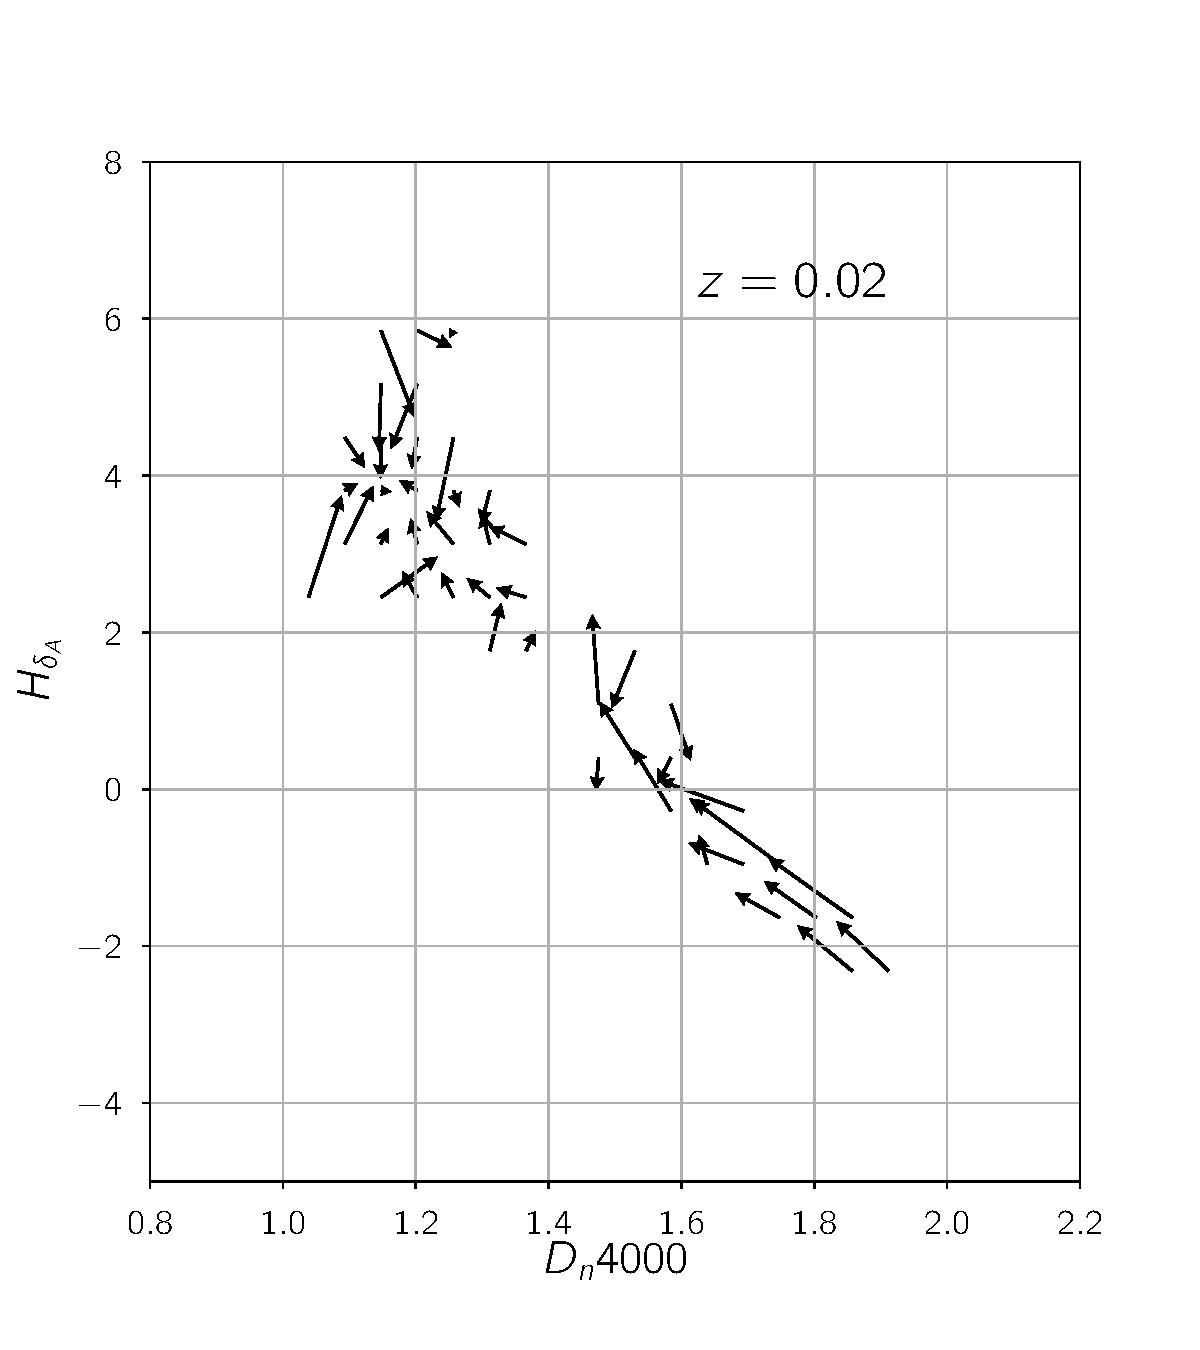
\includegraphics[width=\textwidth]{figures/quiver_a.pdf}
\caption[Short figure name.]{ The mean offset and dispersion in the $h\delta_{A}$ index measured at $z = 0.02,0.06$ and $0.14$ with a $3''$ aperture from the full aperture measurement 
\label{fig:myInlineFigure}}
\end{figure}

\begin{figure}
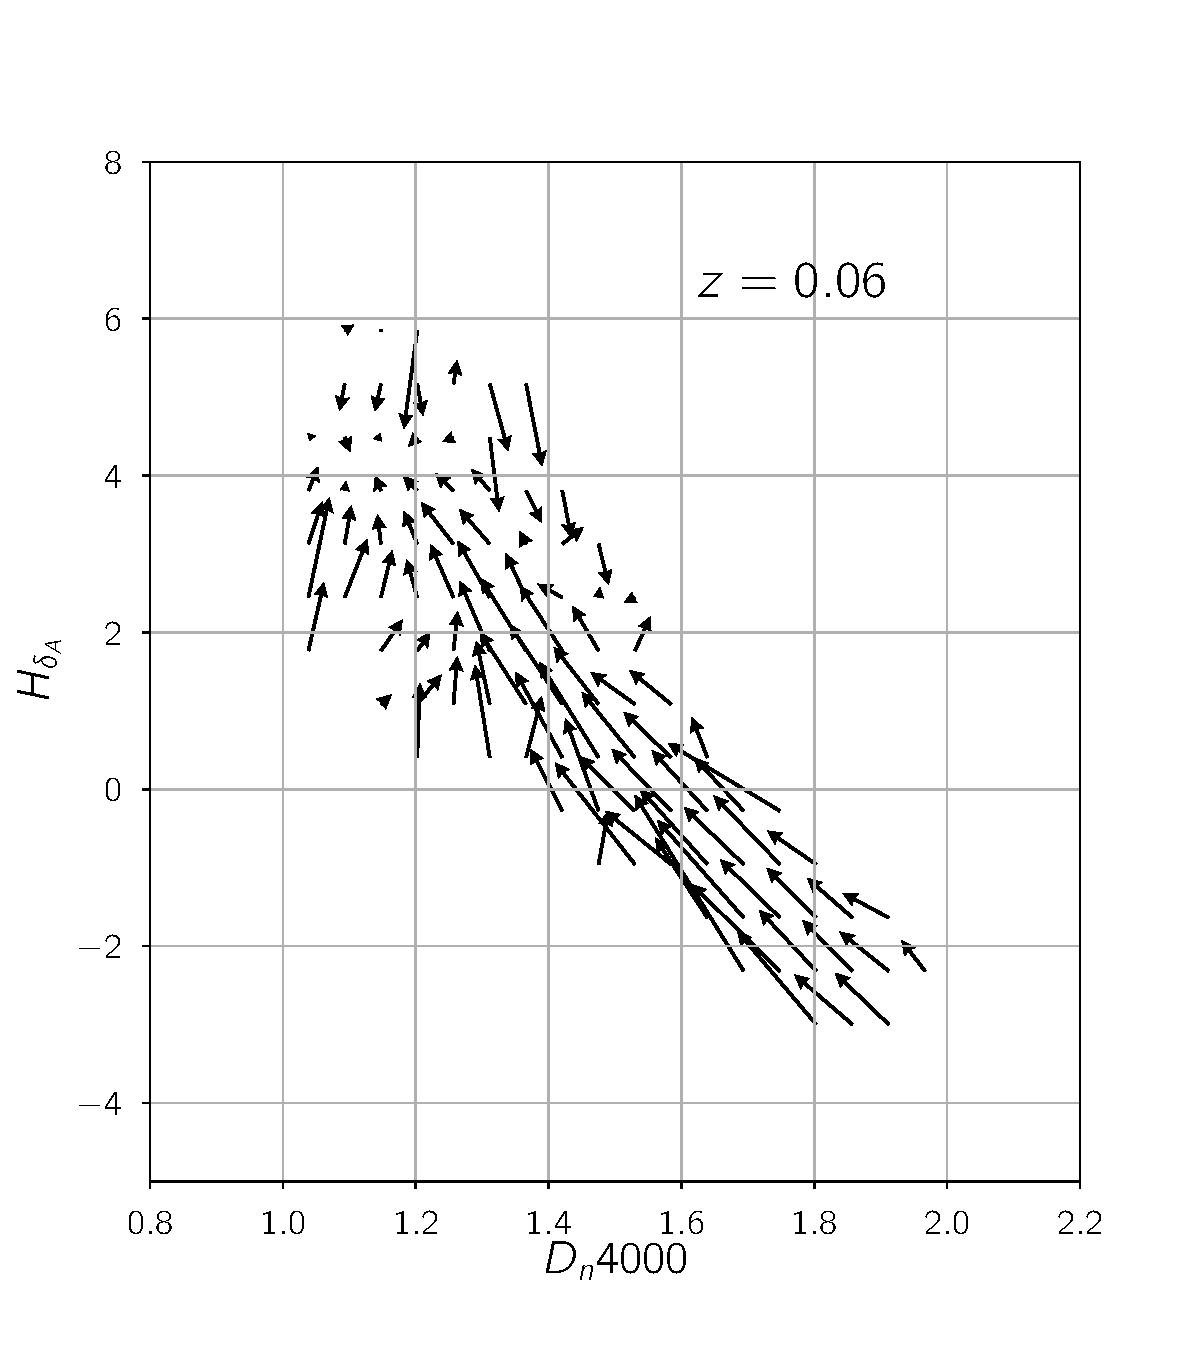
\includegraphics[width=\textwidth]{figures/quiver_b.pdf}
\caption[Short figure name.]{ The mean offset and dispersion in the $h\delta_{A}$ index measured at $z = 0.02,0.06$ and $0.14$ with a $3''$ aperture from the full aperture measurement 
\label{fig:myInlineFigure}}
\end{figure}

\begin{figure}
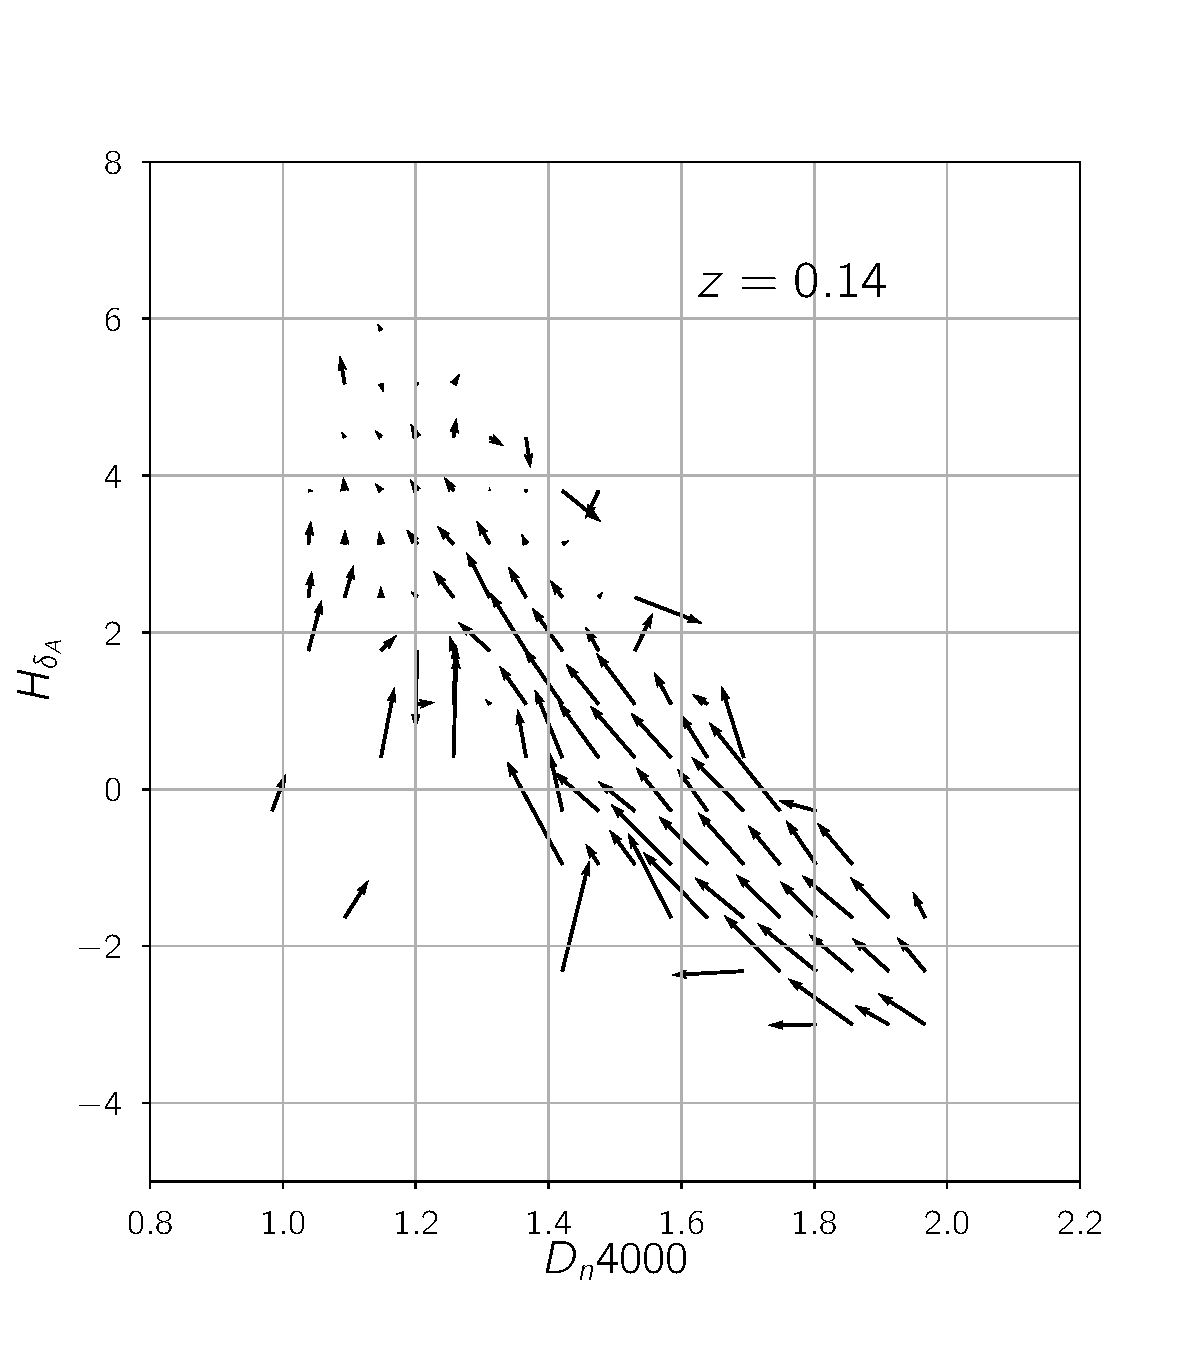
\includegraphics[width=\textwidth]{figures/quiver_c.pdf}
\caption[Short figure name.]{ The mean offset and dispersion in the $h\delta_{A}$ index measured at $z = 0.02,0.06$ and $0.14$ with a $3''$ aperture from the full aperture measurement 
\label{fig:myInlineFigure}}
\end{figure}



